\section{QR decomposition}
\label{sec:QR}

\subsection{Theory}

\subsubsection{Orthogonal matrices}
\label{sec:orthogonalMatrices}
Orthogonal matrices represent either reflections or rotations and fulfill by definition the equations:

\begin{align}
\label{eq:definitionOrthogonal0}
\mathbf{Q}\mathbf{Q}^T = \mathbf{I}\\
\label{eq:definitionOrthogonal1}
\mathbf{Q}^T\mathbf{Q} = \mathbf{I}
\end{align}
%
Therefore, the transposed of an orthogonal matrix is also its inverse:
\begin{align}
\label{eq:orthogonalInverse}
\mathbf{Q}^T = \mathbf{Q}^{-1}
\end{align}
%
Another useful property of orthogonal matrices is, that they preserve the length of a vector during matrix-vector multiplication:
\begin{align}
\label{eq:orthogonalPreserveLength}
\norm{\mathbf{Qx}}= \norm{\mathbf{y}}
\end{align}
%
\subsubsection{Solving linear systems with QR decomposition}

QR decomposition decomposes a matrix $\mathbf{A}$ into an orthogonal matrix $\mathbf{Q}$ and an upper triangular matrix $\mathbf{R}$. 
Solving linear systems with QR decomposition is pretty much straight forward:
\begin{align*}
\mathbf{A}\mathbf{x} &= \mathbf{r}\\
\mathbf{QR}\mathbf{x} &= \mathbf{r}
\end{align*}
%
The product $\mathbf{R}\mathbf{x}$ is substituted by the vector $\mathbf{y}$:

\begin{align*}
\mathbf{Qy} &= \mathbf{r}
\end{align*}
%
Since $\mathbf{Q}$ is orthogonal, it follows:

\begin{align*}
\mathbf{y} &= \mathbf{Q}^{-1}\mathbf{r}\\
\mathbf{y} &= \mathbf{Q}^T\mathbf{r}
\end{align*}
%
The system's solution $\mathbf{x}$ is now obtained by simple backward substitution (see \cref{sec:backwardSubstitution}) because of $\mathbf{R}$ being an upper triangular matrix.
\begin{align*}
\mathbf{R}\mathbf{x} = \mathbf{y}\\
\end{align*}
%
The QR decomposition itself can be calculated with different techniques, namely the Gram-Schmidt process, Givens rotations and Householder reflections.
In this document, Householder reflections are used to calculate the decomposition.
In contrast to the Gram-Schmidt approach, they produce numerically stable results.
Their disadvantage of not being parallelizable is not relevant, since systems which benefit of parallelization are usually to large for a real-time engine.
Givens rotations are much more complex regarding the implementation without offering any real benefit within the scope of small linear systems. 
 

\subsubsection{Householder reflections}

A householder reflection is a reflection at a plane or hyperplane that contains the origin of the coordinate system \draftNoteInline{Add a picture here using pgfplots}.
Because the origin is by definition part of the reflection plane, only its normal $\mathbf{w}$ is needed to describe it mathematically.
The Householder matrix $\mathbf{H}$ which performs the reflection can be calculated as follows:



\begin{align}
\label{eq:HouseholderGeneral}
\mathbf{H} = \mathbf{I} - \frac{2}{\mathbf{w}^T\mathbf{w}}\mathbf{w}\mathbf{w}^T
\end{align}
%
$\mathbf{w}^T\mathbf{w}$ is the scalar product. With $\mathbf{v}$ being the unit normal of the reflection plane

\begin{align*}
	\mathbf{v} = \frac{\mathbf{w}}{\norm{\mathbf{w}}}
\end{align*}
%
\cref{eq:HouseholderGeneral} simplifies to:

\begin{align}
\label{eq:HouseholderGeneral}
\mathbf{H} = \mathbf{I} - 2\mathbf{v}\mathbf{v}^T
\end{align}
%
The Householder matrix $\mathbf{H}$ has some useful properties.
First, it is orthogonal (\cref{sec:orthogonalMatrices}).
Additionally, it is also symmetric, meaning:

\begin{align}
\label{eq:householderSymmetric}
\mathbf{H} = \mathbf{H}^T
\end{align}
%
Combining \cref{eq:householderSymmetric} with \cref{eq:orthogonalInverse} yields:

\begin{align}
\label{eq:householderInverse}
\mathbf{H} = \mathbf{H}^{-1}
\end{align}
%
So a Householder matrix is its own inverse.
Furthermore, abusing the Householder matrix's special structure, the product with another vector or matrix can be computed more efficiently than the standard matrix-vector product or matrix-matrix product:

\begin{align}
\nonumber
\mathbf{H} \mathbf{x}
&= 
\pth{\mathbf{I} - 2\mathbf{v}\mathbf{v}^T}\mathbf{x}
\\&= 
\nonumber
\mathbf{I}\mathbf{x} - 2\mathbf{v}\mathbf{v}^T\mathbf{x}
\\&= 
\label{eq:householderEfficientMatrixVector}
\mathbf{x} - 2\pth{\mathbf{v}^T\mathbf{x}}\mathbf{v}
\end{align}
%
Note that $\mathbf{v}^T\mathbf{x}$ is the scalar product.
Instead of the quadratic complexity of the standard matrix-vector product, \cref{eq:householderEfficientMatrixVector} is only of linear complexity.
For matrix-matrix multiplication the approach is similar and results in quadratic complexity instead of cubic:

\begin{align}
\label{eq:householderEfficientMatrixMatrix}
\mathbf{H} \mathbf{A}
=
\mathbf{A} - 2\mathbf{v}\pth{\mathbf{v}^T\mathbf{A}}
\end{align}
%
$\mathbf{v}^T\mathbf{A}$ is a row vector that contains the scalar products of $\mathbf{v}$ and each column of $\mathbf{A}$

\draftNote{
\begin{itemize}
\item Remember that the calculation of multiple scalar products (calculation of $\mathbf{v}^T\mathbf{A}$) can be vectorized
\end{itemize}
}

\subsubsection{Calculation of a specific Householder reflection}

Consider the case, that two vectors $\mathbf{x}$ and $\mathbf{y}$ of arbitrary length are known and the reflection, which transforms $\mathbf{x}$ in a way that it points into the same direction as $\mathbf{y}$, should be determined.
The equation that describes this problem is:

\begin{align}
\label{eq:housholderCalculateReflection}
\mathbf{H} \mathbf{x} = \lambda \mathbf{y}
\end{align}
%
Since orthogonal matrices preserve a vectors length (see \cref{eq:orthogonalPreserveLength}) it follows:

\begin{align}
\label{eq:housholderCalculateReflectionLambda}
\lambda = \pm \frac{\norm{\mathbf{x}}}{\norm{\mathbf{y}}}
\end{align}
%
So $\lambda$ is the length ratio of the vectors $\mathbf{x}$ and $\mathbf{y}$.
Taking a look at \cref{fig:housholderCalculateReflection} reveals that the difference between the vectors $\mathbf{x}$ and $\mathbf{Hx}$ is orthogonal to the reflection plane.
Therefore, it is a normal of this plane.
Hence, the vector $\mathbf{v}$ of the required Householder reflection can be calculated with:

\begin{align}
\label{eq:housholderCalculateReflectionNormal}
\mathbf{v} = \frac{\mathbf{x} - \lambda \mathbf{y}}{\norm{\mathbf{x} - \lambda \mathbf{y}}}
\end{align}


\begin{figure}
\centering
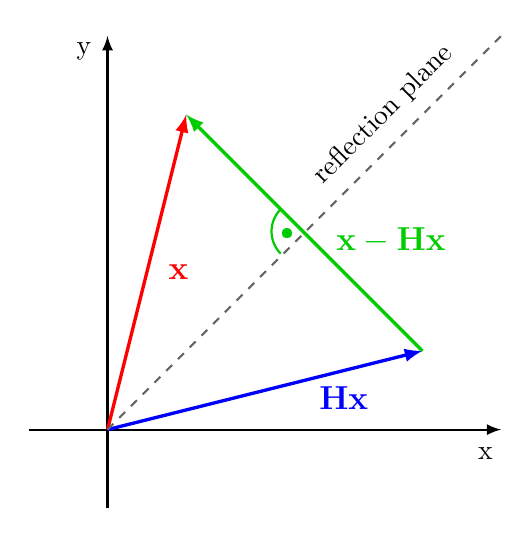
\begin{tikzpicture}
\draw[color=black,-latex,thick] (-1,0)--(5,0);
\draw[color=black,-latex,thick] (0,-1)--(0,5);
\draw[color=red,-latex,very thick] (0,0)--(1,4);
\draw[color=blue,-latex,very thick] (0,0)--(4,1);
\draw[color={black!20!green},-latex,very thick] (4,1)--(1,4);
\draw[color={black!20!green}, thick] (2.2,2.8) arc (135:225:0.4);
\node[color={black!20!green}] at (2.28,2.48) {\textbullet};
\draw[color={black!60!white},dashed,thick] (0,0)--(5,5);
\node[] at (4.8,-0.3) {x};
\node[] at (-0.3,4.8) {y};
\node[color=red] at (0.9,2) {\large{$\mathbf{x}$}};
\node[color=blue] at (3,0.4) {\large{$\mathbf{Hx}$}};
\node[color={black!20!green}] at (3.6,2.4) {\large{$\mathbf{x-Hx}$}};
\node[rotate=45] at (3.5,4) {reflection plane};
\end{tikzpicture}
\caption{Some nice title}
\label{fig:housholderCalculateReflection}
\end{figure}

\subsubsection{Algorithm}

Consider the linear System $\mathbf{Ax} = \mathbf{r}$ with:

\begin{align*}
\mathbf{A}
=
\begin{bmatrix}
a_0&b_0&c_0\\
a_1&b_1&c_1\\
a_2&b_2&c_2
\end{bmatrix}
&&
\mathbf{x}
=
\begin{bmatrix}
x_0\\
x_1\\
x_2
\end{bmatrix}
&&
\mathbf{r}
=
\begin{bmatrix}
r_0\\
r_1\\
r_2
\end{bmatrix}
\end{align*}



